\begin{figure}
\begin{center}
    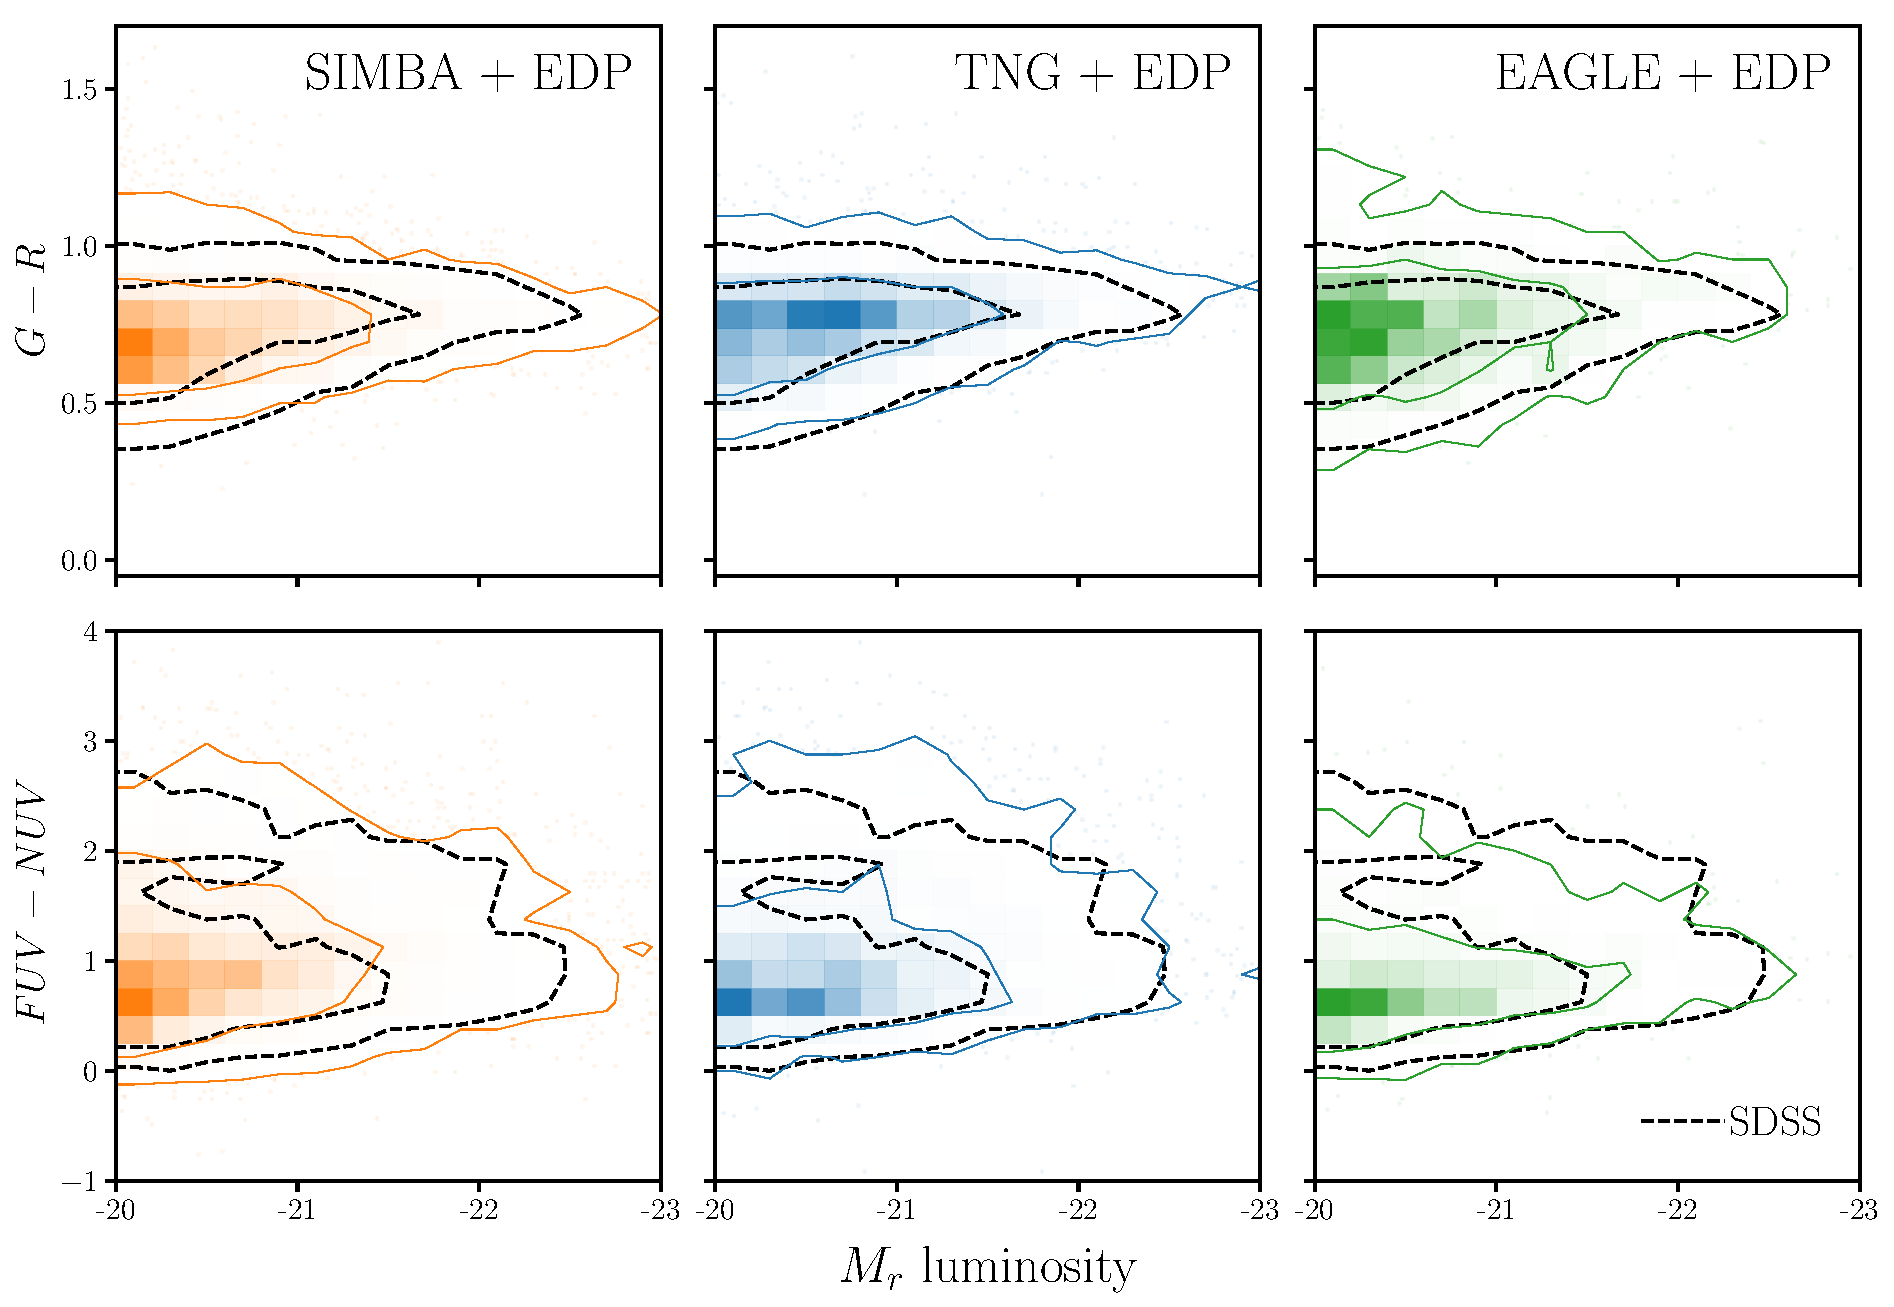
\includegraphics[width=0.9\textwidth]{figs/abc_observables.pdf}
    \caption{\label{fig:dem}
    The optical and UV color-magnitude relations predicted by the DEM with 
    the median ABC posteriors for the SIMBA (orange), TNG (blue), and EAGLE
    (green) hydrodynamical simulations. For comparison, we include the 
    $(\gr) - M_r$ (top panels) and $(\fnuv) - M_r$ (bottom panels) relations
    for SDSS (black dashed). With the DEM, the simulations produce dramatically 
    different observables than when we do not include any dust prescription
    (Figure~\ref{fig:obs}). Hence, dust must be account for when interpreting 
    and comparing simulations. Moreover, with the DEMs, all three simulations
    produce observables consistent with SDSS. Since different simulations can 
    produce reproduce observations by varying dust, dust significantly limits
    our ability to constrain the physical processes that go into galaxy
    simulations. 
    }
\end{center}
\end{figure}


%\begin{figure}
%\begin{center}
%    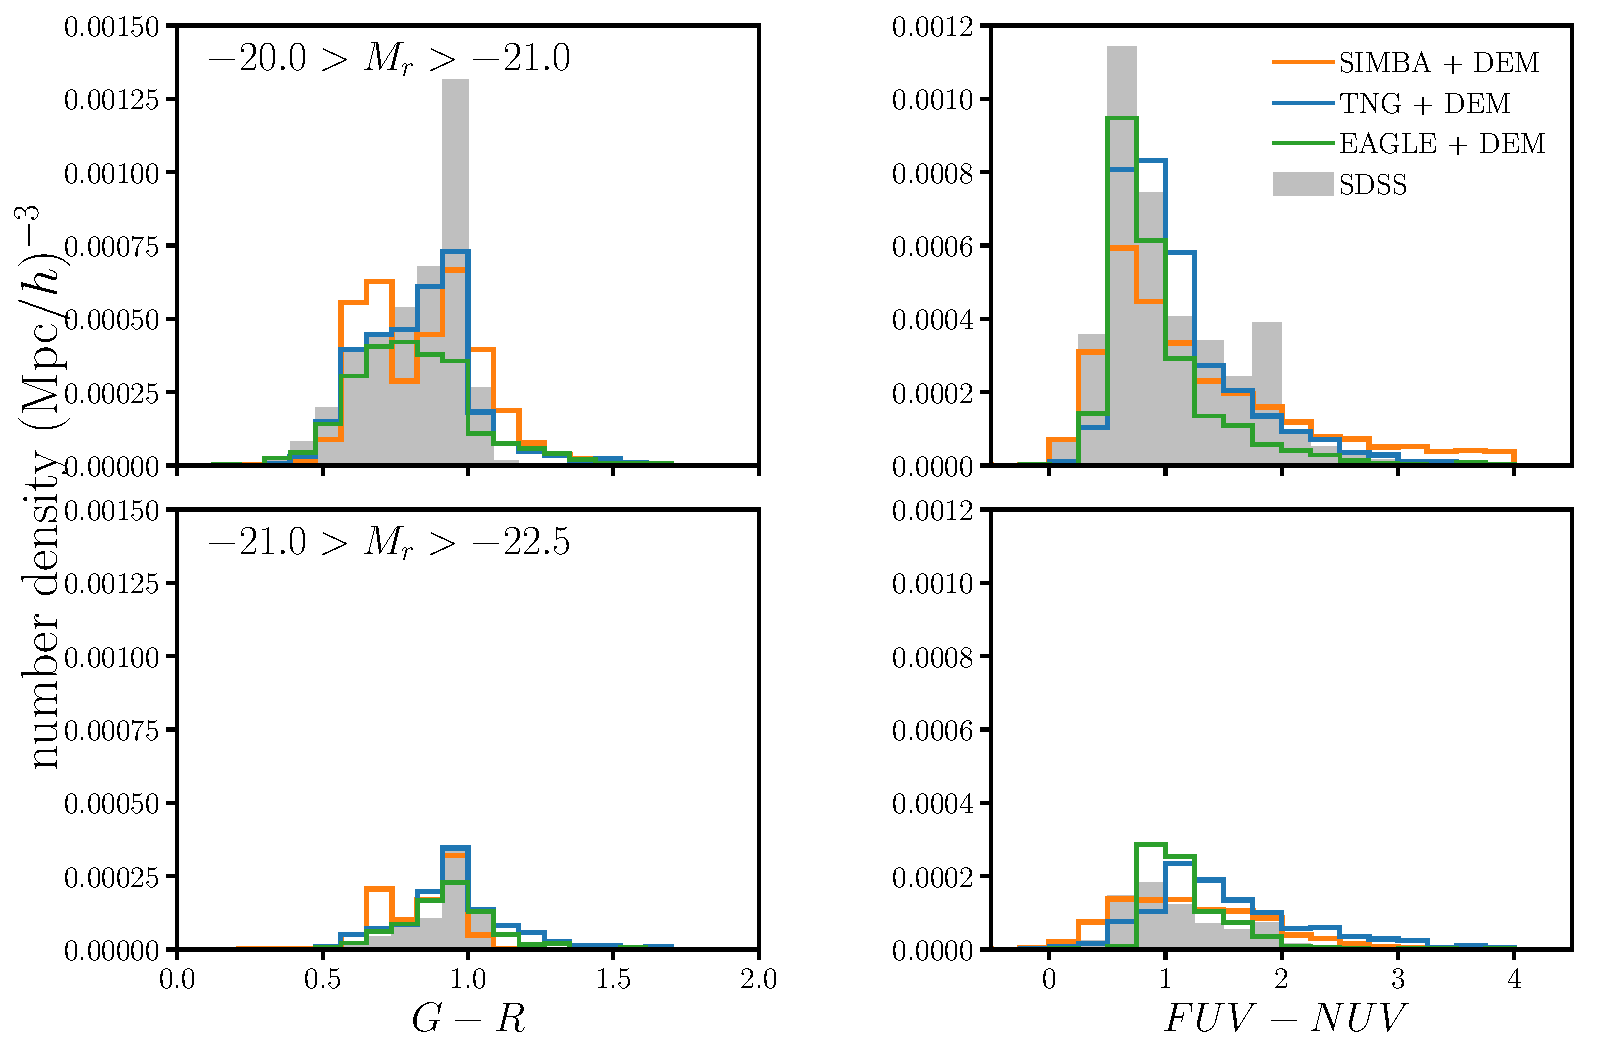
\includegraphics[width=0.85\textwidth]{figs/abc_observables_mr_bin.pdf}
%    \caption{\label{fig:demcloseup}
%    $G-R$ (left) and $FUV-NUV$ (right) number density distributions for the DEM
%    models of the SIMBA (orange), TNG (blue), and EAGLE (green) simulations in
%    two $M_r$ bins: $-20 > M_r > -21$ (top panels) and $-21 > M_r > -22.5$
%    (bottom panels).  Each of the DEM models are run using the median posterior
%    parameter values. In comparison to SDSS (grey shaded), the DEM models predict 
%    consistent red sequence and blue cloud positions in the $G-R$ distributions, 
%    $FUV-NUV$ peak positions, and number density. {\em Overall the DEM
%    models for SIMBA, TNG, and EAGLE produce observables are in good agreement 
%    with SDSS.}
%    }
%\end{center}
%\end{figure}


\section{Results} \label{sec:results}
In Figure~\ref{fig:dem}, we present the optical and UV color-magnitude
relations predicted by the DEM with the median ABC posteriors for the SIMBA
(orange), TNG (blue), and EAGLE (green) simulations. We include the SDSS
observables for comparison (black dashed). Without any dust attenuation, we
previously found that simulations predict dramatically different $(\gr) - M_r$
and $(\fnuv) - M_r$ relations than SDSS (Figure~\ref{fig:obs}). In contrast,
with the DEM, the optical color-magnitude relations have well-defined red
sequences and blue clouds that are consistent with SDSS. The DEM also produces
galaxies with $\fnuv$ distributions that are consistent with SDSS. We
also find good agreement in the galaxy number density at $M_r < -20$:
\ch{numbers} 

% comparison to literature 
% First EAGLE
Previous works in the literature have also compared colors and luminosities
predicted by simulations to observations. For EAGLE, \cite{trayford2015}
calculate colors and luminosities with the {\sc Galaxev} population synthesis
models and a two-component screen model for dust. More recently,
\cite{trayford2017} calculated optical colors for EAGLE using {\sc Skirt}, a
Monte Carlo radiative transfer code~\citep{camps2015}, to model the dust.
Both \cite{trayford2015} and \cite{trayford2017} produce bluer red sequences
compared to GAMA observations, at $10^{11.2} < M_* < 10^{11.5}$ for 
\cite{trayford2017}. Although a detailed comparison is difficult since both works
examine all galaxies, not only centrals, the DEM accurately reproduces the 
position of the SDSS red sequence, even at high $M_*$. \cite{trayford2015} 
also predict significant more luminous blue galaxies than obervations or the DEM. 
Using the same \cite{trayford2017} {\sc Skirt} framework, \cite{baes2019} find
that they overesimtate the observed cosmic spectral energy distributions 
(CSED) in the UV regime. Moreover, the $\fnuv$ color of their CSED is
significantly higher than GAMA $\fnuv$. The DEM, on the other hand, 
predict $\fnuv$ in good agreement with SDSS. 
%\cite{baes2019}: EAGLE+SKIRT SED compparison with GAMA Far UV is not attenuated enough. underrestimates optical and NIR
For TNG, \cite{nelson2018} calculate optical colors using a dust model that
includes attenuation due to dense gas birth clouds surrounding young stellar
populations and also due to simulated distribution of neutral gas and metals.
They find bluer red sequence peaks and a narrower blue cloud compared to SDSS.
Although they compare the color distribution for all galaxies in $M_*$ bins,
we find neither of these discrepancies with the DEM. 
\emph{With the DEM, we produce optical and UV color-magnitude relations that
are in good agreement with observations, better than previous works, for the
SIMBA, TNG, and EAGLE hydrodynamical simulations.}

Figures~\ref{fig:dem} clearly illustrates that any comparison of simulations 
must include dust attenuation. Dust dramatically changes the predicted 
observables of simulations. Without dust (Figure~\ref{fig:obs}), we did 
not find a clearly bimodality in the optical color-magnitude relation and
the simulations predicted UV colors outside of the range of observations.
But with a simple framework for dust motivated by attenuation laws and 
correlation with galaxy properties, such as the DEM, simulations can 
reproduce observations. Our results also highlight another key point. Robustly interpreting subgrid
physics in simulations requires marginalizing over dust. Even for three
simulations that produce significantly different SMFs and $M_*-\sfr$ relations
(Figure~\ref{fig:smf_msfr}), the DEM is able to produce observables that agree
with observations. In fact for SIMBA, the DEM reproduces the observations by assigning
higher attenuation to star-forming galaxies so that they populate the red sequence 
while quiescent galaxies populate the blue cloud. This is due to the large
number of low mass star-forming SIMBA galaxies that lie well above the SFS
(Figure~\ref{fig:smf_msfr}), which would otherwise all be luminous blue
galaxies not found in observations. Our current understanding of dust, which is
encapsulated in the DEM, has enough flexiblity to reproduce observations 
for simulations that predict galaxy populations with different physical
properties, even if it means contradicting the established relationship 
between color and $\sfr$. Then marginalizing over dust would leave little 
constraining power on the subgrid galaxy physics of the simulations. 
Therefore, \emph{current limitations in our understanding of dust in 
galaxies significant impedes our ability to investigate galaxy 
formation from simulations.}

% what we learn about AV - galaxy property connection  
In addition to reproducing observations, DEM also provides insight into dust in
galaxies. Given the parameterization of the DEM, it is especially easy to
interpret correlation between dust attenuation and galaxy physical properties.
In all three simulations, we find significant positive $M_*$ dependence of
$\tau_V$, $\mtaum \sim 2$ (Figure~\ref{fig:abc}), consistent with previous
works in the literature. \cite{burgarella2005}, for instance, found significant
positive $M_*$ dependence in $FUV$ attenuation in NUV-selected and FIR-selected
samples. \cite{garn2010} and \cite{battisti2016} also find positive $M_*$ 
dependence in SDSS star-forming galaxies. Most recently, \cite{salim2018} 
find higher $V$ and $FUV$ attenuation for more masssive star-forming galaxies in the
GALEX-SDSS-WISE Legacy Catalog 2 (GSWLC2). 
In addition to the $M_*$ dependence, the DEM posteriors also reveal the
correlation between dust attenuation and star formation. Ignoring SIMBA, which
flips the color versus $\sfr$ relation, we find $\mtaus\sim-1$ --- galaxies 
with lower $\sfr$ have higher attenuation. Observations that examine the
relationship between dust attenuation and $\sfr$~\citep[\eg][]{garn2010,
reddy2015, battisti2016, battisti2017, salim2018} have thus far focused
primarily on star-forming galaxies. With the DEM, we confirm that 
\emph{galaxies with higher $M_*$ have overall higher dust attenuation
and find that galaxies with lower $\sfr$ have overall higher dust attenuation}. 

%They find that
%star-forming galaxies with higher SFR have higher attenuation; however, this
%trend is driven by the $M_*$ dependence since star-forming galaxies lie on 
%the star-forming sequence~\citep{garn2010, battisti2017}. At fixed $M_*$,
%observations find no strong $\sfr$ dependence for the star-forming population. 
%Since previous works do not include quiescent galaxies, %\cite{tress2018} find positive dependence between E(B-V) (color excess) with M* and negative dependence with
%SSFR for 1753 star-forming galaxies within 1.5 < z < 3.  

%For instance, \cite{garn2010} find that SDSS star-forming galaxies with higher
%SFR have higher H$\alpha$ attenuation. \cite{battisti2016} find a consistent
%correlation for the Balmer optical depth of star-forming galaxies in GALEX and SDSS 
%using 10000 SF galaxies GALEX-SDSS. Although at higher redshifts,  
%\cite{reddy2015} also find this correlation among $z{\sim}2$ star-forming galaxies of
%MOSFIRE Deep Evolution Field.

%\cite{battisti2017} using 5000 SF galaxies from found little stellar mass dependence in the opposite direction (less attenuation at higher stellar masses). But they have big error bars and only probe up to 9.7
%\cite{reddy2015} SF galaxies from $z\sim2$ MOSFIRE Deep Evolution Field survey find strong correlation with SFR. %ionized gas is more reddened relative to the stellar continuum with increasing SFR 

\begin{figure}
\begin{center}
    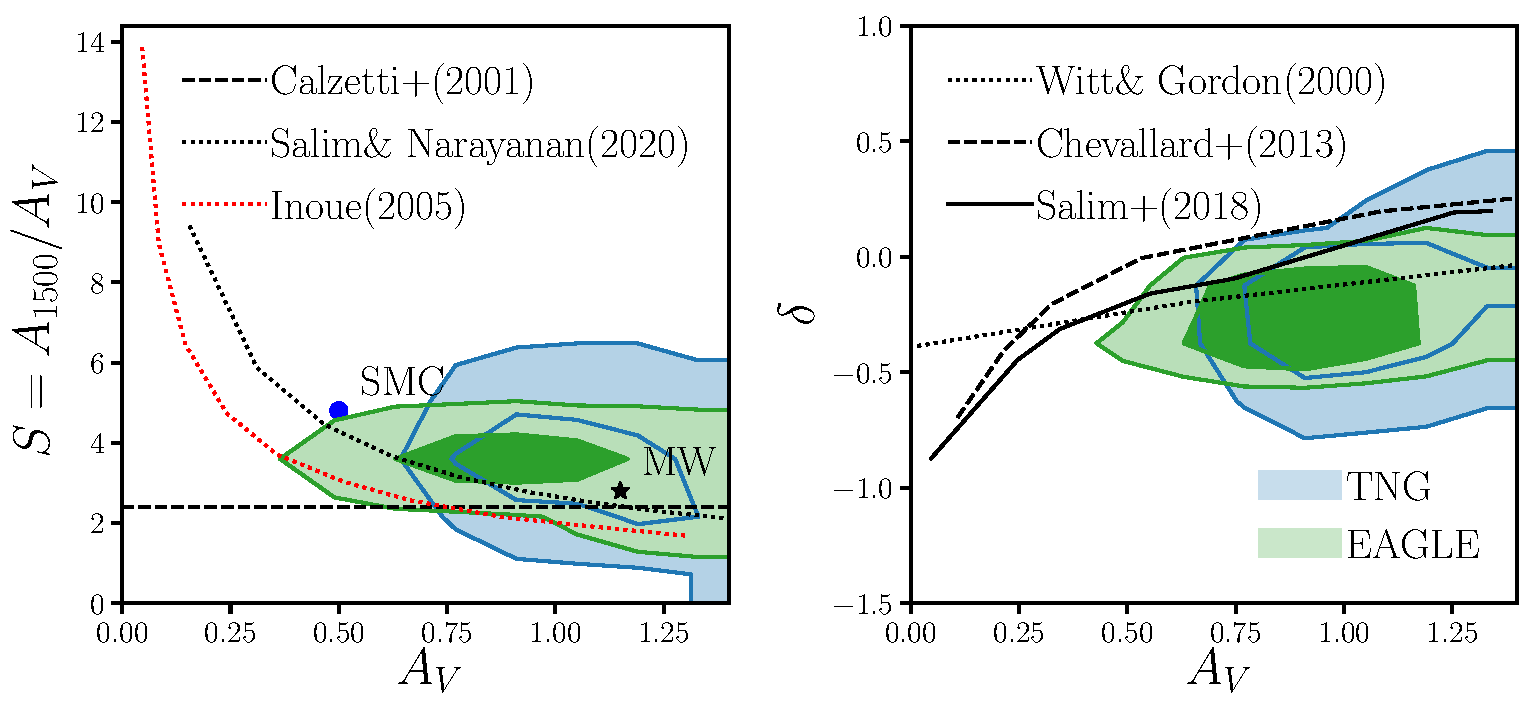
\includegraphics[width=0.85\textwidth]{figs/abc_slope_AV.pdf}
    \caption{\label{fig:slope}
    The attenuation-slope relation for TNG (blue) and EAGLE (green) simulations
    with the DEM. We present the relation usng two different measurements of slope, 
    commonly used in the ltierature: $S = A(1500\AA)/A_V$ (left panel) and
    the slope offset from the \cite{calzetti2001} curve, $\delta$ (right panel).
    The DEM moodels predict an attenuation-slope relation, where the slope is
    steeppr at lower attenuation, consistent with both observations and
    simulation. The DEM models only include masssive galaxies, hence, they do
    not include mnay galaxies with low attenuatiton. At $A_V > 0.5$, however, 
    the DEM models are in good agreement with observations~\cite{salim2020}. In
    fact, the DEM models match the observed attenuation-slope relation 
    better than radiative transfer simulations, which predict attenuation 
    curves that are too shallow~\citep{inoue2005, chevallard2013, trayford2020}
    }
\end{center}
\end{figure}

% attenuation curve slope  
Our results also shed light on the slope of dust attenuation. In Figure~\ref{fig:slope}, 
we present the attenuation-slope relation for TNG (blue) and EAGLE (green) with the DEM.
The left and right panels present two different measurements of the slope $S =
A(3000\AA)/A_V$, which is easier to cosntrain in observations, and $\delta$,
the slope offset from the \cite{calzetti2001} curve that use in the DEM. 
We include the attenuation and slope for the Milky Way (star) for reference.
TNG and EAGLE both predict slopes within $2 < S < 5$ and centered around $S\sim
3.5$. In comparison, for the same $A_V > 0.4$ range as the DEM, observations 
find slopes within the range $2 < S < 5$~\citep{calzetti2000, burgarella2005, johnson2007,
conroy2010b, wild2011, battisti2016, battisti2017, leja2017, salim2018} in good
agreement. We also find that the DEM predicts steeper attenuation curves at 
lower attenuation. This is consistent with the established attenuation--slope
relation. At low attenuation, dust scattering dominates absoprtion so the 
attenuation curve steepens because red light scatters isotropically while blue light
scatters forward~\citep{gordon1994, witt2000, draine2003}. %, which causes more optical-to-IR light to escape the galaxy than UV light
At high attenuation dust absorption is dominant and the attenuation curve is
shallower~\citep{chevallard2013}. For the $A_V$ range probed by the DEM, the
$A_V$--slope relation is in good agreement with GSWLC2 galaxies~\citep[black shaded][]{salim2020}.
They are also consistent with \cite{leja2017}. We also compare our results to
theoretical predictions from radiative transfer models, \cite{inoue2005}
(dotted), the radiative transfer models considered in \cite{chevallard2013}
(dot dashed), and \cite{trayford2020} (light shaded), which all predict shallower 
attenuation curves than observations. This is also the case for the
\cite{narayanan2018} attenuation curves (not included). 
Overall, \emph{the dust attenuation curve slopes from the DEM for are in
excellent agreement with observations and better reproduces the observed
attenuation--slope relation than radiative transfer models.}

%We can also examine the correlation between attenuation curve slopes and galaxy properties with the DEM. For TNG and EAGLE, we find that 
%\cite{leja2017} find composite and AGN galaxies generally have shallower  
%slopes, although their sample is limited to only 129 galaxies, In contrast,
%\cite{salim2018} find that quiescent galaxies in the GALEX-SDSS-WISE Legacy
%Catalog 2~\citep[GSWLC2;][]{salim2019} have significantly steeper curves. They,
%however, also find significantly steeper curves for the starburst population 
%(\ie~galaxies above the SFS). With no consensus in the literature and few
%observations that examine the correlation between $\delta$ and galaxy
%properties, the lack of $M_*$ and $\sfr$ dependence we find on $\delta$ is an
%interesting prediction for future observations. 


%\cite{calzetti2000} find  slopes of $2.3 < S < 2.9$ for low-redshift starburst galaxies, 
%\cite{burgarella2005} find $2.5 < S < 6.2$ for 50 UV and 100 IR selected galaxies,
%\cite{johnson2007} find $S\sim2.5$ for 1000 nearby galaxies, 
%\cite{conroy2010} find $S\sim4.5$ for 3400 $10^{9.5} < M_* < 10^{10} M_\odot$ disk galaxies,
%\cite{wild2011} find $2.5 < S < 4.5$ for 23,000 $z{\sim}0.07$ star-forming galaxies, 
%\cite{battisti2016, battisti2017} find slopes consistent with Calzetti (S=2.4) for SF galaxies 
%\cite{leja2017} 130 relatively massive galaxies 2 < S < 15
%\cite{salim2018} 230,000 SDSS galaxies 2 < S < 15 with median S = 5.4
% high z
%\cite{kriek2013}  using stacked SEDs of medium- and broadband photometry of
%galaxies at 0.5 < z < 2 find an average slope of delta=-0.2  but they restrict
%to galaxies with moderate to high optical attenuations (AV> 0.5), 
%\cite{salmon2016} is also spot on. 


% attenuation-slope relation 

%\cite{trcka2020}: EAGLE+SKIRT with CIGALE to get physical properties of
%galaxies. trcka2020 compares to dustpedia~\citep{davies2017} They lok at
%IRX-beta relation.

\begin{figure}
\begin{center}
    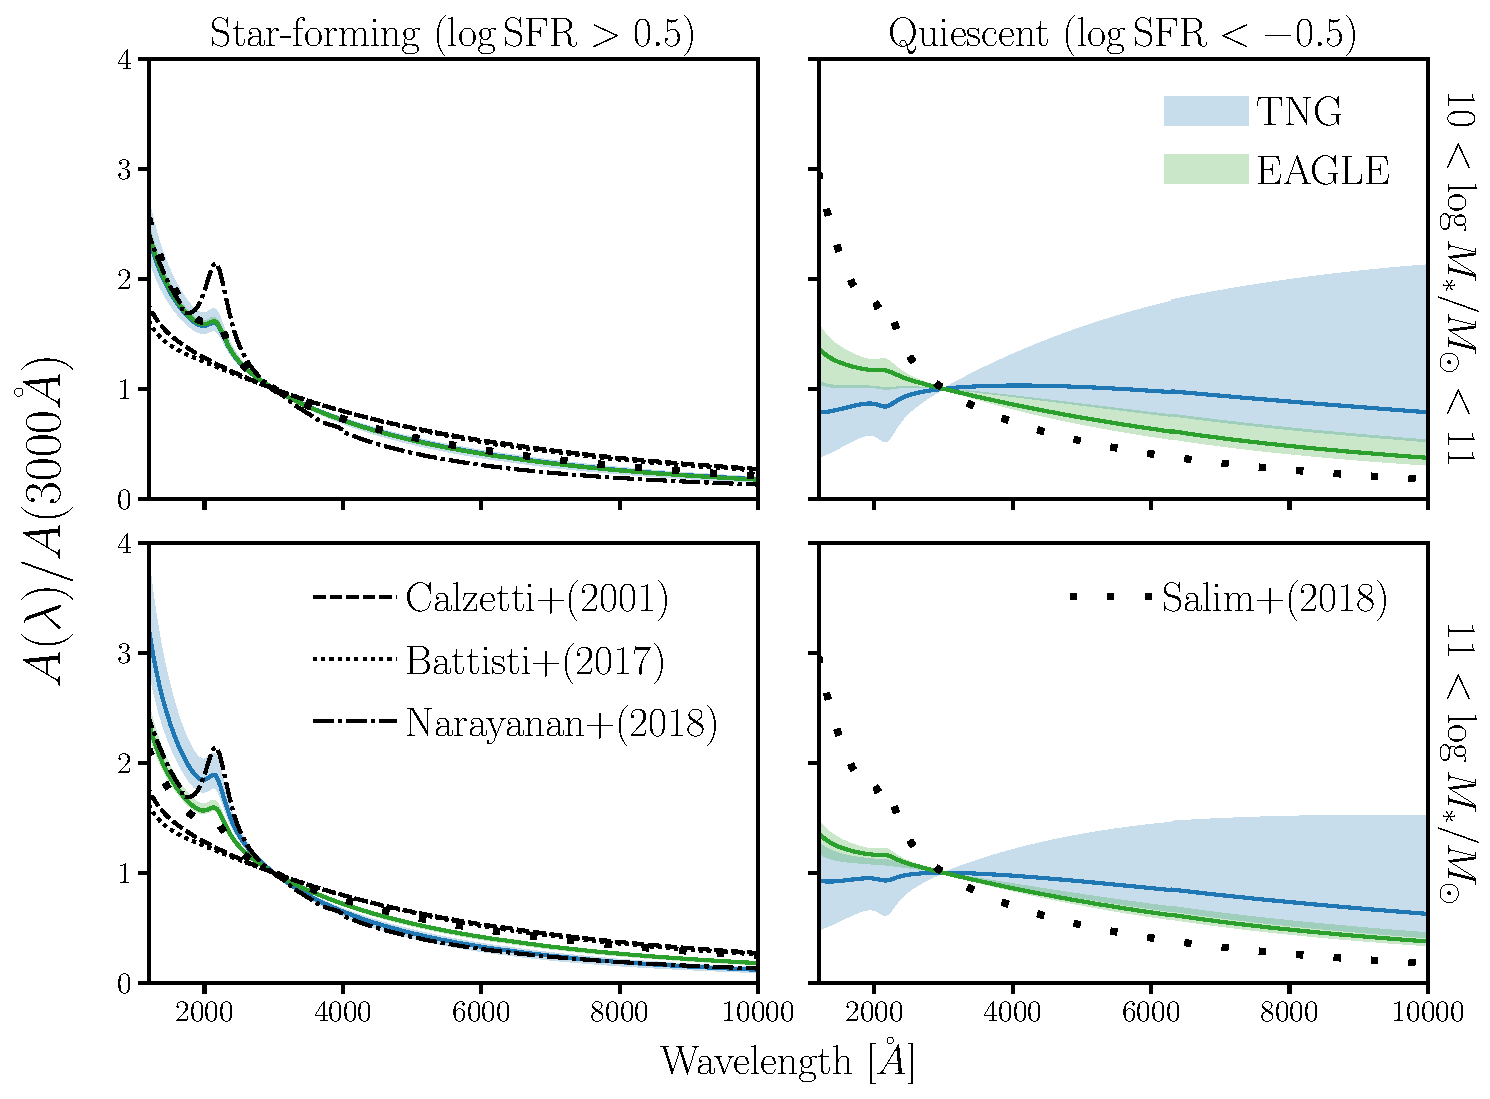
\includegraphics[width=0.85\textwidth]{figs/abc_attenuation.pdf}
    \caption{\label{fig:atten}
    Attenuation curves of the TNG (blue) and EAGLE (green) DEM models for 
    low (top) and high $M_*$ (bottom), star-forming (left) and
    quiescent galaxies (right). The attenuation curves are normalized at
    $3000\AA$: $A(\lambda)/A(3000\AA)$. We mark the $1\sigma$ standard
    deviation of the attenuation curves with the shaded region. For comparison,
    we include measurements of $A(\lambda)/A(3000\AA)$ from 
    observations~\citep{caleztti2000, battisti2017, salim2018} as well as
    from simulations~\citep{narayanan2018}. For star-forming galaxies, the 
    \cite{calzetti2000} and \cite{battisti2017} attenuation curves are shallower 
    than the DEM attenuation curves; however, this is primarily driven by the
    differences in $M_*$ ranges. For \cite{salim2018}, which probe a similar
    $M_*$ range as our DEM models, we find goood agreement. We also find good 
    agreement with median attenuation curve of \cite{narayanan2018}. With DEM
    models, we can also constrain the attenuation curves of quiescent galaxies,
    which are challenging to observationally constrain. Quiescent galaxies,
    have significantly shallower attenuation curves with larger variations in
    slope. 
    }
\end{center}
\end{figure}

% variation of attenuation curve  
In Figure~\ref{fig:atten}, we present the normalized attenuation curves of the TNG
(blue) and EAGLE (green) DEM for low (top) and high $M_*$ (bottom),
star-forming (left) and quiescent galaxies (right). The attenuation curves are
normalized at $3000\AA$ in order to emphasize their slopes. Also, although the
DEM does not model the complexities of dust-star geometry, it includes
significant variations in the dust attenuation through the slab model
and the dependence on galaxy properties, which we present with the
shaded region (1$\sigma$ standard deviation about the median). For comparison, 
we include $A(\lambda)/A(3000\AA)$ from observations~\citep{calzetti2000, battisti2017, salim2018} 
as well as from simulations~\citep{narayanan2018}. The \cite{calzetti2000} and
\cite{battisti2017} attenuation curves are derived from $M_* < 10^{9.9}M_\odot$ 
star-forming galaxies. Meanwhile, the \cite{salim2018} curves are for
star-forming galaxies with $10^{9.5} < M_* < 10^{10.5}M_\odot$ star-forming
galaxies (top left) and $10^{10.5} < M_*M_\odot$ star-forming galaxies (bottom
left). 

The attenuation curves for star-forming centrals in TNG and EAGLE are in good 
agreement with the \cite{salim2018} curves as well as the median curve of
\cite{narayanan2018} star-forming galaxies. They are, however, steeper than 
the \cite{calzetti2000} and \cite{battisti2017} curves. Figure~\ref{fig:atten} 
also reveals a possible $M_*$ dependence in the slopes, especially for TNG.
Lower $M_*$ star-forming galaxies have slightly shallower attenuation curves.
If this $M_*$ dependence of $\delta$ in the DEM extends below our $M_*$ range, 
we expect a better agreement the \cite{calzetti2000} and \cite{battisti2017} 
curves as well. Besides their slopes, we also find significant variations in
$A(\lambda)$. This is generally consistent with \cite{salim2018} and
\cite{narayanan2018}. They present larger variations; however, this is due to
their broader $M_*$ range. Our results imply that even among star-forming
galaxies with similar $M_*$, there is significant variation in their attenuation
curves.

%\ch{what do we learn about quiescent galaxy attenuation?} 
The DEM also sheds light on dust attenuation in quiescent galaxies, which is
particularly valuable since there are many challenges to measuring attenuation
curves for quiescent galaxies in observations. For instance, methods that rely
on IR luminosities can be contaminated by MIR emission from AGN heating nearby
dust~\cite{kirkpatrick2015}. Even SED fitting methods require accounting for
AGN MIR emission~\citep{salim2016, leja2018, salim2018} in addition to the
challenge in breaking the degeneracy between SFH and metallicity to fit the
continuum (\ch{cite?}). With the DEM, which foward models optical and UV
photometry, we do not face these issues. For both TNG and EAGLE, quiescent
galaxies have shallower attenuation curve with large variations in the slopes
(Figure~\ref{fig:atten}). They also have higher $A_V \gtrsim 1.25$. 
\ch{explanation for why DEM model does this} 

%In \cite{leja2017}, they similar find composite and AGN galaxies
%to have shallow attenuation curves with higher $A_V$; however, the comparison
%is limited due to ther smaller sample size (129 galaxies). In contrast,  
%\cite{salim2018} find that quiescent galaxies in GSWLC2 have significantly
%steeper curves; they, however, focus their analysis mainly on star-forming 
%galaxies.

% Kartheik on why dust is hard to constrain for quiescent galaxies: 
%firstly because quiescent galaxies don't have much recent SFR and therefore not much dust (their most recently produced dust has likely happened more than a dust destruction timescale ago), 
% secondly because the continuum for quiescent galaxies is super hard to fit (and break degeneracies with SFH & metallicity), which leads to poor(er) constraints. You could basically think of this in terms of dust/total SNR, which drops sharply for this population.

The DEM produces optical and UV color-magnitude relations overall consistent
with SDSS and also reveals key insight into dust attenuation in galaxies. There
are, however, still a few discrepancies between the DEM observables and SDSS.
For instance, the DEM produces broader distributions overall observations.
Galaxies in SDSS sharply cut-off above the red sequence, while some galaxies in
the DEM broadly extend beyond the cut-off. The DEM also produces galaxies 
more luminous galaxies than SDSS. Nevertheless, the DEM better reproduces
observations than other works. Furthermore, we chose linear relations to
parameterize $\tau_V$ and $\delta$ in the DEM for simplicity. However, the
empirical framework of the DEM can easily be extended to more flexible
parameterizations that better reproduce observations --- the only challenge
would be to find a well-motivated parameterization from observations.

In the DEM, we make a few other assumptions and choices. For simulated galaxies
with $\sfr=0$, we directly sample their observables from the distributions of 
SDSS quiescent galaxies. These $\sfr=0$ galaxies do not have recent
star-formation and also have 0 gas mass\todo{CHH: @tjitske is this for all
sims} so we would expect them to also have no dust. However, without
attenuating these galaxies, the simulations struggle to reproduce observations.
Our prescription for $\sfr = 0$ galaxies ensures that $\sfr=0$ galaxies do not
impact our results, without delving into the issue further. In
Appendix~\ref{sec:res}, we describe our prescription in detail and discuss the
limitations of the simulations near the mass and temporal resolutions or their
gas prescriptions. Another assumption in the DEM is how we assign $A_V$ using 
the slab model (Eq.~\ref{eq:slab}). Although the slab model is consistent with
the correlation between attenuation and inclination in
observations~\citep[\eg][]{conroy2010b, salim2020} and
simulations~\citep[\eg]{chevallard2013, narayanan2018, trayford2020} and
reproduces the SDSS $A_V$ distribution (Figure~\ref{fig:av_dist}),
we test the robustness of our results by replacing it with a more flexible
truncated normal distribution in Appendix~\ref{sec:nonslab}. Replacing the slab
model, does not significantly impact our results. We therefore conclude that
our results are robust to the assumptions and choices we make in the DEM. 

% Salim(2020): Chevallard et al. (2013), who aggregated and analyzed a diverse series of theoretical attenuation law studies by Pierini et al. (2004), Tuffs et al. (2004), Silva et al. (1998) and Jonsson et al. (2006), and showed that all the stud- ies predict, with some normalization differences, a relationship between the optical depth AV and attenuation law slope.

% Salmon+(2016): There is evidence that galaxy inclination correlates with the strength of Lyα emission, such that we observe less Lyα equivalent width for more edge-on galaxies (Charlot & Fall 1993; Laursen & Sommer-Larsen 2007; Yajima et al. 2012; Verhamme et al. 2012; U et al. 2015)
% Therefore, based on physi- cal models, one expects that galaxies with “greyer” dust laws and larger overall attenuation should have higher inclinations
% Salim+(2018): Chevallard et al. (2013) furthermore show that the depend- ence of the slope on AV is the same irrespective of whether the AV is driven by different levels of intrinsic (face-on) attenuation or is the result of inclined viewing geometry. 

% recap what we learn from the  
In this work, we present the DEM, an empirical framework for including dust
attenuation in simulated galaxy populations. We apply the DEM to the SIMBA,
TNG, and EAGLE hydrodynamical simulations and forward model optical and UV
color-magnitude relations. %Then we compare the forward modeled DEM outputs to SDSS observations to reveal insights into the simulations as well as dust attenuation in galaxies.
For all three simulations, we reproduce SDSS observations with the DEM.
However, based on the inferred DEM parameter posteriors, we find that 
SIMBA requires an extreme dust attenuation that reverses the established 
relationship between color and $\sfr$. SIMBA overpredicts a large starburst
population at $<10^{10}M_\odot$ and otherwise struggles to reproduce
observations. \todo{any specific subgrid physics in SIMBA that's responsible}.

Focusing on the DEM for TNG and EAGLE, we find significant $M_*$ and $\sfr$
dependences in the amplitude of dust attentuation, $A_V$. More massive
galaxies have higher dust attenuation; galaxies with lower 
$\sfr$ have  higher dust attenuation. Also, we find that the DEM attenuation
curves closely reproduce the observed attenuation--slope relation, better than
radiative transfer models. Furthermore, the DEM produces attenuation curves
that are in good agreement with the literature for star-forming galaxies and is
able to constrain the attenuation curves for quiescent galaxies, which have few
constraints from observations. Based on these attenuation curves, quiescent
galaxies have shallower attenuation curves than star-forming galaxies. Lastly,
we find significant variation in the attenuation curves even for galaxies with
comparable $M_*$ and $\sfr$.

By reproducing SDSS observations with the DEM for different hydrodynamical
simulations, we demonstrate that accounting for dust attenuation is essential 
to reproduce observations. However, based on our current understanding of dust
there is enough flexiblity to reproduce observations even for simulations that
predict galaxy populations with significantly different physical properties. Since adjusting dust alone
can reproduce observations, dust is highly degenerate with the variations in
subgrid physics across simulations. In other words, if we were to marginalize
over dust we would not be able to differentiate between the various
hydrodyanmical models using observations. So detailed comparisons across
simulations and to observations likely overinterpret the differences and
similarities found in simulations. Therefore, the current limitations in our
understanding of dust is a major bottleneck for investigating galaxy formation
using simulations.

The DEM provides a simple empirical model for applying dust attenuation to
galaxies. With only a few parameters, it allows $M_*$ and $\sfr$ dependences in
dust attenuation curves, reproduces the attenuation--slope relation, and
produces attenuation curves with significant variation. Combined with a
simulation-based inference method such as ABC-PMC, it provides a direct
framework for inferring dust attenuation from observations. Upcoming
surveys such as the Bright Galaxy Survey of the Dark Energy Spectroscopic
Instrument~\citep[DESI;][\ch{Ruiz\etal2020}](desicollaboration2016), 
the Galaxy Evolution Survey of the Prime Focus
Spectrograph~\citep[PFS;][]{takada2014,tamura2016}, and the Wide-Area VISTA
Extragalactic Survey~\citep[WAVES;][]{driver2016, driver2019} will provide
more statistically powerful observations to tightly constrain dust
attentuation. For those uninterested in dust, the DEM provides a
straightforward framework for marginalizing over dust. \todo{IQ3 description?} 
